% AUTOR_LIVRO_EDICAO.tex
% Preencher com o nome das cor ou composição RGB (ex: [r=0.862, g=0.118, b=0.118]) 
\usecolors[crayola]                   % Paleta de cores pré-definida: wiki.contextgarden.net/Color#Pre-defined_colors

% Cores definidas pelo designer:
% MyGreen          r=0.251, g=0.678, b=0.290 % 40ad4a
% MyCyan          r=0.188, g=0.749, b=0.741 % 30bfbd
% MyRed               r=0.820, g=0.141, b=0.161 % d12429
% MyPink          r=0.980, g=0.780, b=0.761 % fac7c2
% MyGray          r=0.812, g=0.788, b=0.780 % cfc9c7
% MyOrange          r=0.980, g=0.671, b=0.290 % faab4a

% Configuração de cores
\definecolor[MyColor][VividViolet]      % ou ex: [r=0.862, g=0.118, b=0.118] % corresponde a RGB(220, 30, 30)
\definecolor[MyColorText][white]     % ou ex: [r=0.862, g=0.118, b=0.118] % corresponde a RGB(167, 169, 172)


\def\MyCoverCenter#1{\starttikzpicture[overlay, remember picture]
              \node
                   [draw=none, 
                    blur shadow={shadow xshift=5.5pt,shadow yshift=-1.5pt, shadow scale=0.93},
                    shadow opacity=50, 
                    shadow blur extra rounding] 
                    at (0.45  \textwidth,-.25\textheight) {\externalfigure[#1][width=3cm]};
                \stoptikzpicture}


\def\MySecondCover#1{\starttikzpicture[overlay, remember picture]
              \node
                   [draw=none, 
                    blur shadow={shadow xshift=5.5pt,shadow yshift=-1.5pt, shadow scale=0.93},
                    shadow opacity=50, 
                    shadow blur extra rounding] 
                    at (0.70  \textwidth,-.3\textheight) {\externalfigure[#1][width=2.6cm]};
                \stoptikzpicture}

% Classe para diagramação dos posts
\environment{marketing.env}             

\starttext %---------------------------------------------------------|

\Mensagem{PROJETO LUIZ GAMA}

\startMyCampaign

\hyphenpenalty=10000
\exhyphenpenalty=10000

{\bf AGORA SOMOS FINALISTAS DO JABUTI}
\stopMyCampaign

\MyCoverCenter{GAMA_DIREITO_THUMB}
%\vfill\scale[lines=1.5]{\MyStar[MyColorText][none]}
\starttikzpicture[remember picture,overlay]
\node[text=white] at (4.2,-5.5) {\Seta\,{\bf ORG.} BRUNO RODRIGUES DE LIMA};
\stoptikzpicture

\starttikzpicture[remember picture,overlay]
\node at (5.5,-3.2) {\externalfigure[JABUTI.png][width=2cm]};
\stoptikzpicture

% \node at (8.5,-6)
% {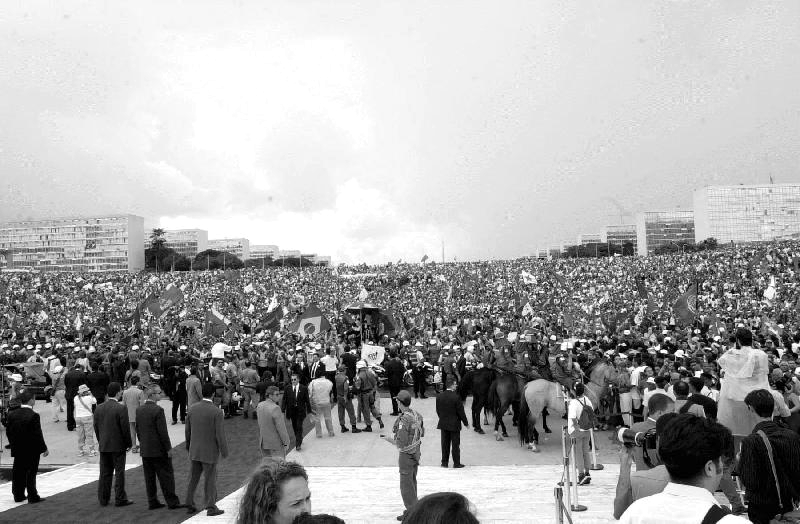
\includegraphics[height=\textheight]{midia/1.jpg}};

 \page %---------------------------------------------------------| 

\hyphenpenalty=10000
\exhyphenpenalty=10000

«Para nós, os democratas, a abolição da escravatura é essencialmente social; para os verdadeiros cristãos é fraternal e religiosa; para os capitalistas é monetária, cambial e econômica; perante Deus, porém, a escravidão é um {\bf CRIME HORRENDO}.»

{\vfill\scale[factor=6]{\Seta\,{\bf Luiz Gama}, Direito.}}

\page %---------------------------------------------------------|

\Hedra

\stoptext %---------------------------------------------------------|




% A religião, a moral, o direito e a liberdade são gêneros deteri-��orados que não têm cotação nos mercados do Império.Aí compra-se e vende-se o homem; açoitam-se-lhe as carnes,monetariza-se-lhe o suor e o sangue, o homem é o escravo, oescravo é o dinheiro e a questão é essencialmente econômica!

